% Makros zur Kompatibilitaet mit Onlinemodul: 
 \providecommand{\MoIl}[1][]{\mbox{}#1]\mathopen{}} 
 \providecommand{\MoIr}[1][]{#1[\mbox{}} 
 \providecommand{\MIntvlSep}{;} 
 \providecommand{\MElSetSep}{\, ; \, } 
 \begin{MAufgabe}{Lineare Betrags(un)gleichungen}{vr, 2016, MaTeX}
L\"osen Sie die Gleichung
$$
 \MDS 5\left| 2\, x + 2 \right|3 - x= 3 \left| 2\, x - 4 \right| 4 - 3\, x
$$  

\ifLsg\MLoesung

Im ersten Schritt k\"onnen die Terme au\ss{}erhalb der Betragszeichen zusammengefasst werden:

\begin{align*} 
 5\left| 2\, x + 2 \right|3 - x= 3 \left| 2\, x - 4 \right| 4 - 3\, x\\ 
\Leftrightarrow2\, x + 5\, \left|2\, x + 2\right| - 3\, \left|2\, x - 4\right| - 1= 0 
 \end{align*}

F\"ur diese Gleichung haben wir 4 F\"alle zu unterscheiden: 
\begin{enumerate}
\item $ \MDS 
\begin{cases} 
 0 \leq 2\, x + 2\\ 
0 \leq 2\, x - 4
 \end{cases}
\Leftrightarrow 2 \leq x\Leftrightarrow x \in [ 2 \, \MIntvlSep \, \infty\MoIr $ 
\item $ \MDS 
\begin{cases} 
 0 \leq 2\, x + 2\\ 
2\, x - 4 < 0
 \end{cases}
\Leftrightarrow x < 2 \wedge -1 \leq x\Leftrightarrow x \in [ -1 \, \MIntvlSep \, 2\MoIr $ 
\item $ \MDS 
\begin{cases} 
 2\, x + 2 < 0\\ 
0 \leq 2\, x - 4
 \end{cases}
 \mbox{ : keine L\"osung. Diese Bedingung ist nirgendwo erf\"ullt.}$ 
\item $ \MDS 
\begin{cases} 
 2\, x + 2 < 0\\ 
2\, x - 4 < 0
 \end{cases}
\Leftrightarrow x < -1\Leftrightarrow x \in \MoIl  -\infty \, \MIntvlSep \, -1\MoIr $ 
\end{enumerate} 
Der 3. Fall ist nirgendwo erf\"ullt. Betrachte weiter nur die restlichen F\"alle.
 
 Fallunterscheidung: 

 \begin{enumerate} 
 \item Sei $ \MDS x\in[ 2 \, \MIntvlSep \, \infty\MoIr $. 
 In diesem Fall gilt: 
  $ \MDS \left| 2\, x + 2\right|=2\, x + 2$ und $ \MDS \left| 2\, x - 4\right|=2\, x - 4$. \\ 
 Damit ist die Gleichung 
 $$ 
2\, x + 5\, \left|2\, x + 2\right| - 3\, \left|2\, x - 4\right| - 1= 0
$$
 \"aquivalent zur Gleichung
 $$ 
5\left(2\, x + 2\right)-3\left( 2\, x - 4\right)+2\, x-1= 0 
$$  
$$ 
 \Leftrightarrow 6\, x + 21= 0 
$$  
$$ \Leftrightarrow x = - \frac{7}{2} . 
 $$ 
 Die L\"osung muss auch die Fallbedingung $x\in [ 2 \, \MIntvlSep \, \infty\MoIr  $ erf\"ullen. Die gefundene L\"osung $x=- \frac{7}{2}$ erf\"ullt die Fallbedingung  $x\in [ 2 \, \MIntvlSep \, \infty\MoIr $ nicht und deshalb ist  $$
 \mathcal{L}_{1}=\emptyset 
 $$ 
\item Sei $ \MDS x\in[ -1 \, \MIntvlSep \, 2\MoIr $. 
 In diesem Fall gilt: 
  $ \MDS \left| 2\, x + 2\right|=2\, x + 2$ und $ \MDS \left| 2\, x - 4\right|=4 - 2\, x$. \\ 
 Damit ist die Gleichung 
 $$ 
2\, x + 5\, \left|2\, x + 2\right| - 3\, \left|2\, x - 4\right| - 1= 0
$$
 \"aquivalent zur Gleichung
 $$ 
5\left(2\, x + 2\right)-3\left( 4 - 2\, x\right)+2\, x-1= 0 
$$  
$$ 
 \Leftrightarrow 18\, x - 3= 0 
$$  
$$ \Leftrightarrow x = \frac{1}{6} . 
 $$ 
 Die L\"osung muss auch die Fallbedingung $x\in [ -1 \, \MIntvlSep \, 2\MoIr  $ erf\"ullen. Die gefundene L\"osung $x=\frac{1}{6}$ erf\"ullt die Fallbedingung  $x\in [ -1 \, \MIntvlSep \, 2\MoIr $ und deshalb ist  $$
 \mathcal{L}_{2}=\left\{\frac{1}{6}\right\}
 $$ 
\item Sei $ \MDS x\in\MoIl  -\infty \, \MIntvlSep \, -1\MoIr $. 
 In diesem Fall gilt: 
  $ \MDS \left| 2\, x + 2\right|= - 2\, x - 2$ und $ \MDS \left| 2\, x - 4\right|=4 - 2\, x$. \\ 
 Damit ist die Gleichung 
 $$ 
2\, x + 5\, \left|2\, x + 2\right| - 3\, \left|2\, x - 4\right| - 1= 0
$$
 \"aquivalent zur Gleichung
 $$ 
5\left( - 2\, x - 2\right)-3\left( 4 - 2\, x\right)+2\, x-1= 0 
$$  
$$ 
 \Leftrightarrow  - 2\, x - 23= 0 
$$  
$$ \Leftrightarrow x = - \frac{23}{2} . 
 $$ 
 Die L\"osung muss auch die Fallbedingung $x\in \MoIl  -\infty \, \MIntvlSep \, -1\MoIr  $ erf\"ullen. Die gefundene L\"osung $x=- \frac{23}{2}$ erf\"ullt die Fallbedingung  $x\in \MoIl  -\infty \, \MIntvlSep \, -1\MoIr $ und deshalb ist  $$
 \mathcal{L}_{3}=\left\{- \frac{23}{2}\right\}
 $$ 
 \end{enumerate} 
  Die L\"osungsmenge des Ausgangsproblems ist die Vereinigung der einzelnen L\"osungsmengen: 
$$ \mathcal{L} = \mathcal{L}_{1} \cup \mathcal{L}_{2} \cup \mathcal{L}_{3} 
 = \emptyset\cup \left\{\frac{1}{6}\right\}\cup \left\{- \frac{23}{2}\right\} 
  =\left\{\frac{1}{6}\right\}\cup\left\{- \frac{23}{2}\right\} 
  = \left\{\frac{1}{6}\MElSetSep- \frac{23}{2}\right\} 
 . $$ 
 
 \begin{center}
 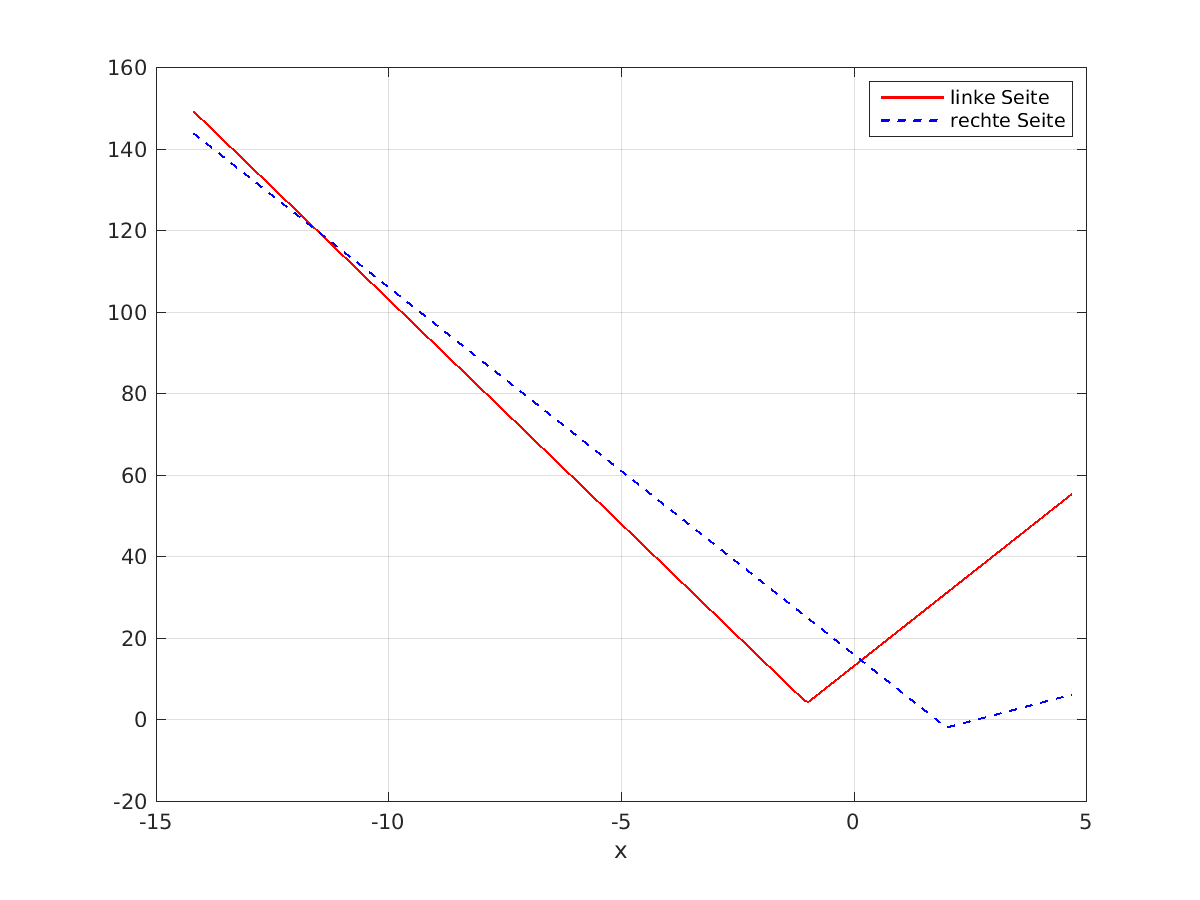
\includegraphics[width=0.8\linewidth]{Abb_zur_Ag_autogenerated_ineq_2.png} \end{center}
 
\else\relax\fi
 \end{MAufgabe}